%!TEX root = main.tex

\section{Introduction}
\label{sec:intro}

During recent years, \gh (2008) has become the largest code host in the world, with more than 5M developers
collaborating across 10M repositories.
Due to its support for distributed version control (Git) and pull-based development~\cite{barr2012cohesive},
as well as its modern Web UI and focus on social coding~\cite{dabbish2012social}, \gh has surpassed in size
and popularity even much older forges such as Sourceforge (1999).
As a result, numerous projects (especially open source) are migrating their code base to \gh (for instance,
the Google query \emph{migrate to github} returns more than 4M results), which now hosts popular projects
such as Ruby on Rails, Homebrew, Bootstrap, Django or jQuery.

Researchers have quickly jumped on board and have started exploring \gh data.
So far, studies focused on
building language models of source code~\cite{allamanis2013mining},
understanding the effects of branching and pull-based software development~\cite{lee2013git, gousios2014exploratory},
uncovering associations between crowdsourced knowledge and software development~\cite{vasilescu2013stackoverflow},
visualizing collaboration and influence~\cite{heller2011visualizing},
exploring the social network of developers~\cite{thung2013network, schall2013follow, jiang2013understanding},
or investigating how the social nature of \gh impacts collaboration and impression formation~\cite{dabbish2012social, marlow2013impression}
and could be used to improve development practices~\cite{pham2013creating, pham2013building}.
More studies are expected to be published this year, since \gh is the topic of the Mining Challenge
at the 2014 edition of the Working Conference on Mining Software Repositories (MSR).
However, as opposed to Stack Overflow (also 2008), the largest Q\&A site for programming-related questions
and the topic of the Mining Challenge at the 2013 edition of MSR, the richness of \gh data remains
largely underexplored in terms of academic publications~\cite{vasilescu2012meta}.

To facilitate studies of \gh, we have created \ght~\cite{gousios2012ghtorrent}, %, gousios2013ghtorent}, 
a scalable,
queriable, offline mirror of the data offered through the \gh REST API.
\ght data has already been used in empirical studies (e.g., \cite{gousios2014exploratory, squire2014forge,
vasilescu2013stackoverflow}).
%, and a subset of it has been selected as the topic of the Mining Challenge
%at the 2014 edition of the Working Conference on Mining Software Repositories (MSR).
%In response to feedback received from \ght users after its official release~\cite{gousios2013ghtorent},
In this paper we present a novel feature designed to offer customisable data dumps on demand.
The new \ght data-on-demand service offers users the possibility to request via a web form up-to-date \ght
data dumps (in both MySQL and MongoDB formats) for any collection of \gh repositories.

Apart from lowering the ``barrier for entry'' even further for researchers interested in mining \gh data,
this data-on-demand service offers several advantages.
Firstly, while the \ght project already offered data dumps of both its raw data (MongoDB, currently more than 2TB)
and metadata (MySQL, currently more than 20GB), downloading and restoring these dumps can be
very time consuming and might not be necessary if a particular analysis is restricted in scope to say a handful
of ``interesting'' \gh projects (e.g., the Ruby on Rails project, for which separate data sets also started being
collected~\cite{wagstrom2013network}).

\begin{figure*}[t]
\begin{center}
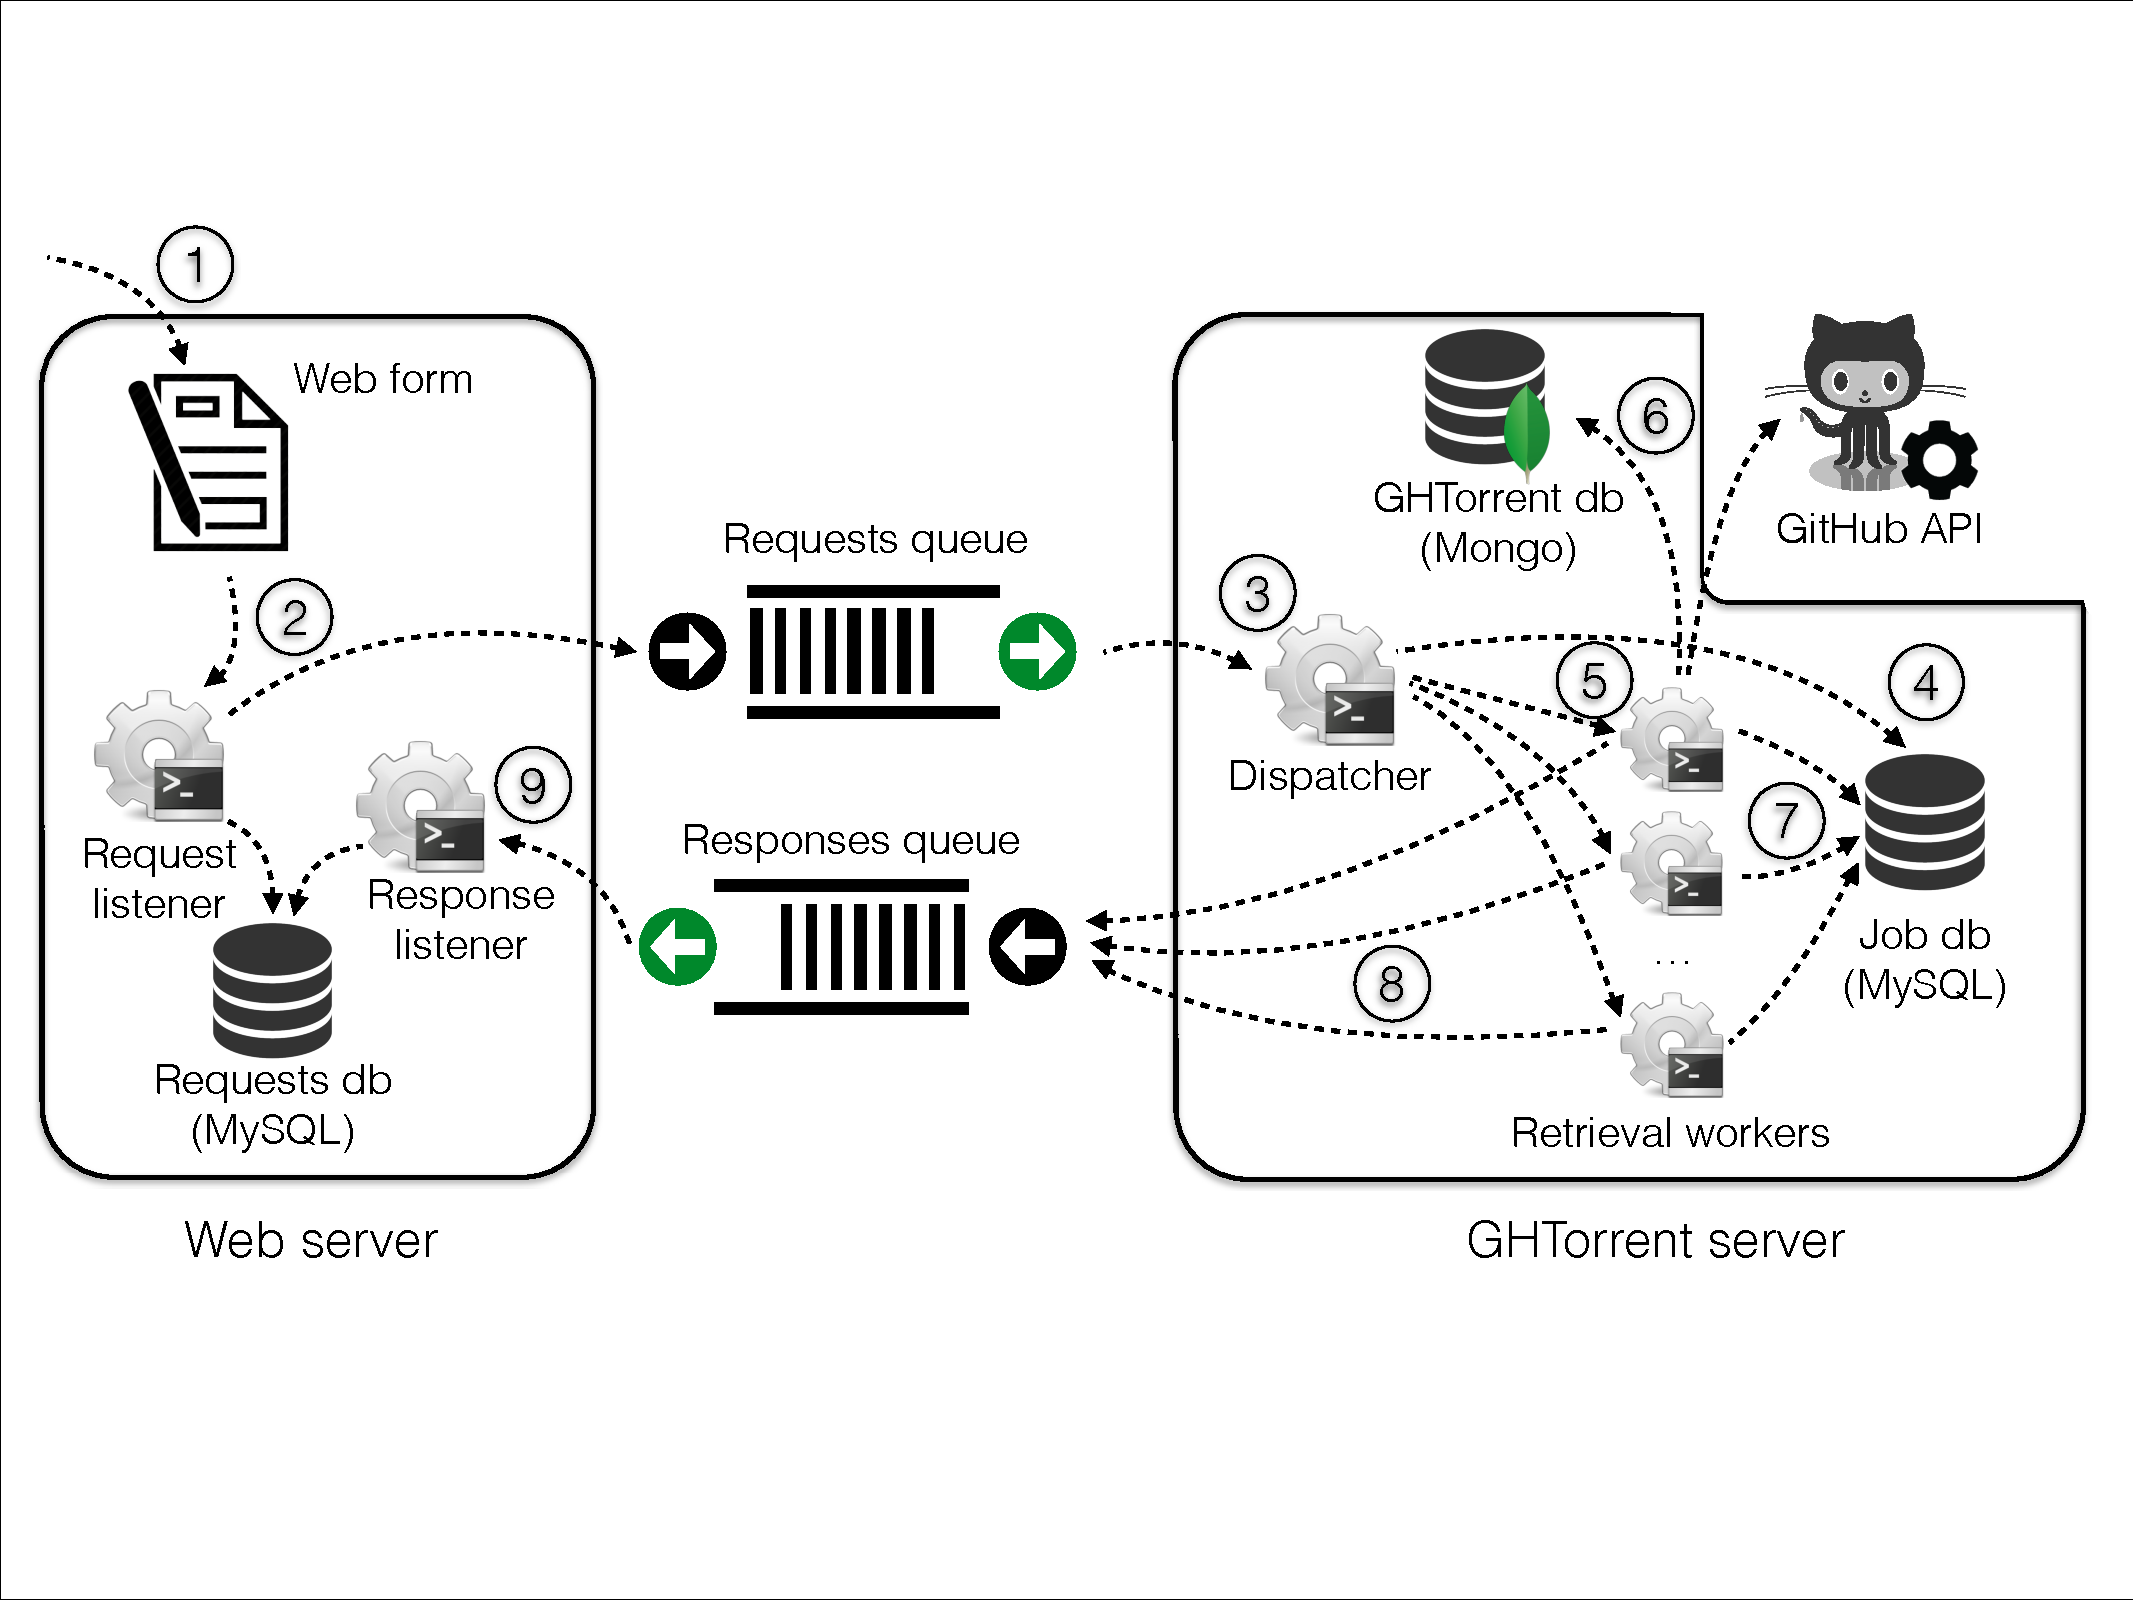
\includegraphics[width=0.9\textwidth, trim=5 160 5 105, clip=True]{figures/architecture.pdf}
\caption{Architecture of the \ght data-on-demand service.}
\label{fig:architecture}
\end{center}
\end{figure*}

Secondly, while the idea of running queries with a restricted scope is not necessarily new with respect to
the official release of \linebreak \ght~\cite{gousios2012ghtorent}, the data-on-demand service enhances replicability
of results obtained using \ght data.
\ght already offered an online query interface with access to an archived version of the relational database,
which could be used to restrict the scope of a query.
However, \gh is a very dynamic platform where developers, projects and wikis are created and deleted constantly.
Therefore, online queries of \ght data may return different results at different times if project data recorded
by \ght has been refreshed in the meantime.
To enhance the replicability~\cite{gonzalez2012reproducibility} of such results, it is therefore preferable to
store the exact snapshot of the data set used in the analysis.

Thirdly, our experiences with curating academic papers based on Stack Exchange data~\cite{vasilescu2012meta}
suggest that researchers prefer to work with data dumps rather than online data explorers
(for reasons such as eliminating the reliance on a third party service, replicability, or integration with existing
tooling or infrastructure).
Even after factoring out papers published at the Mining Challenge of MSR 2013, an overwhelming
fraction of the remaining Stack Exchange papers published after 2010 (when the Stack Exchange data explorer
became available) have used data dumps rather than the data explorer.
We hope that by offering customisable \ght data dumps we will encourage researchers to intensify their efforts
to mine \gh data.

The rest of this paper is organised as follows.
In Section~\ref{sec:arch} we describe the architecture of lean \ght, followed by a discussion of how to use the
service in Section~\ref{sec:usage}.
Next, we discuss related work in Section~\ref{sec:relwork}, and present our conclusions in Section~\ref{sec:conclusions}.

